%!TEX root = ../chapter3.tex
%******************************
%	 Results 
%*****************************

\section{Droplet based single-cell RNA sequencing of mouse testis}
\subsection*{High-resolution profiling by single-cell RNA-seq captures the unidirectional differentiation of germ cells during adult spermatogenesis}

Spermatogenesis is a recurrent differentiation process that produces male gametes within testicular seminiferous tubules \textbf{(Fig. \ref{fig3:cell_types}A)}. The seminiferous epithelium in the mouse is classified into twelve distinct stages, based on the combination of cell types present \textbf{(Fig. \ref{fig3:cell_types}B)}. Tubules cycle asynchronously and continuously through these stages and adult testis contain tubules in every possible epithelial stage \textbf{(Fig. \ref{fig3:cell_types}}. \\

\begin{figure}[!h]
\centering
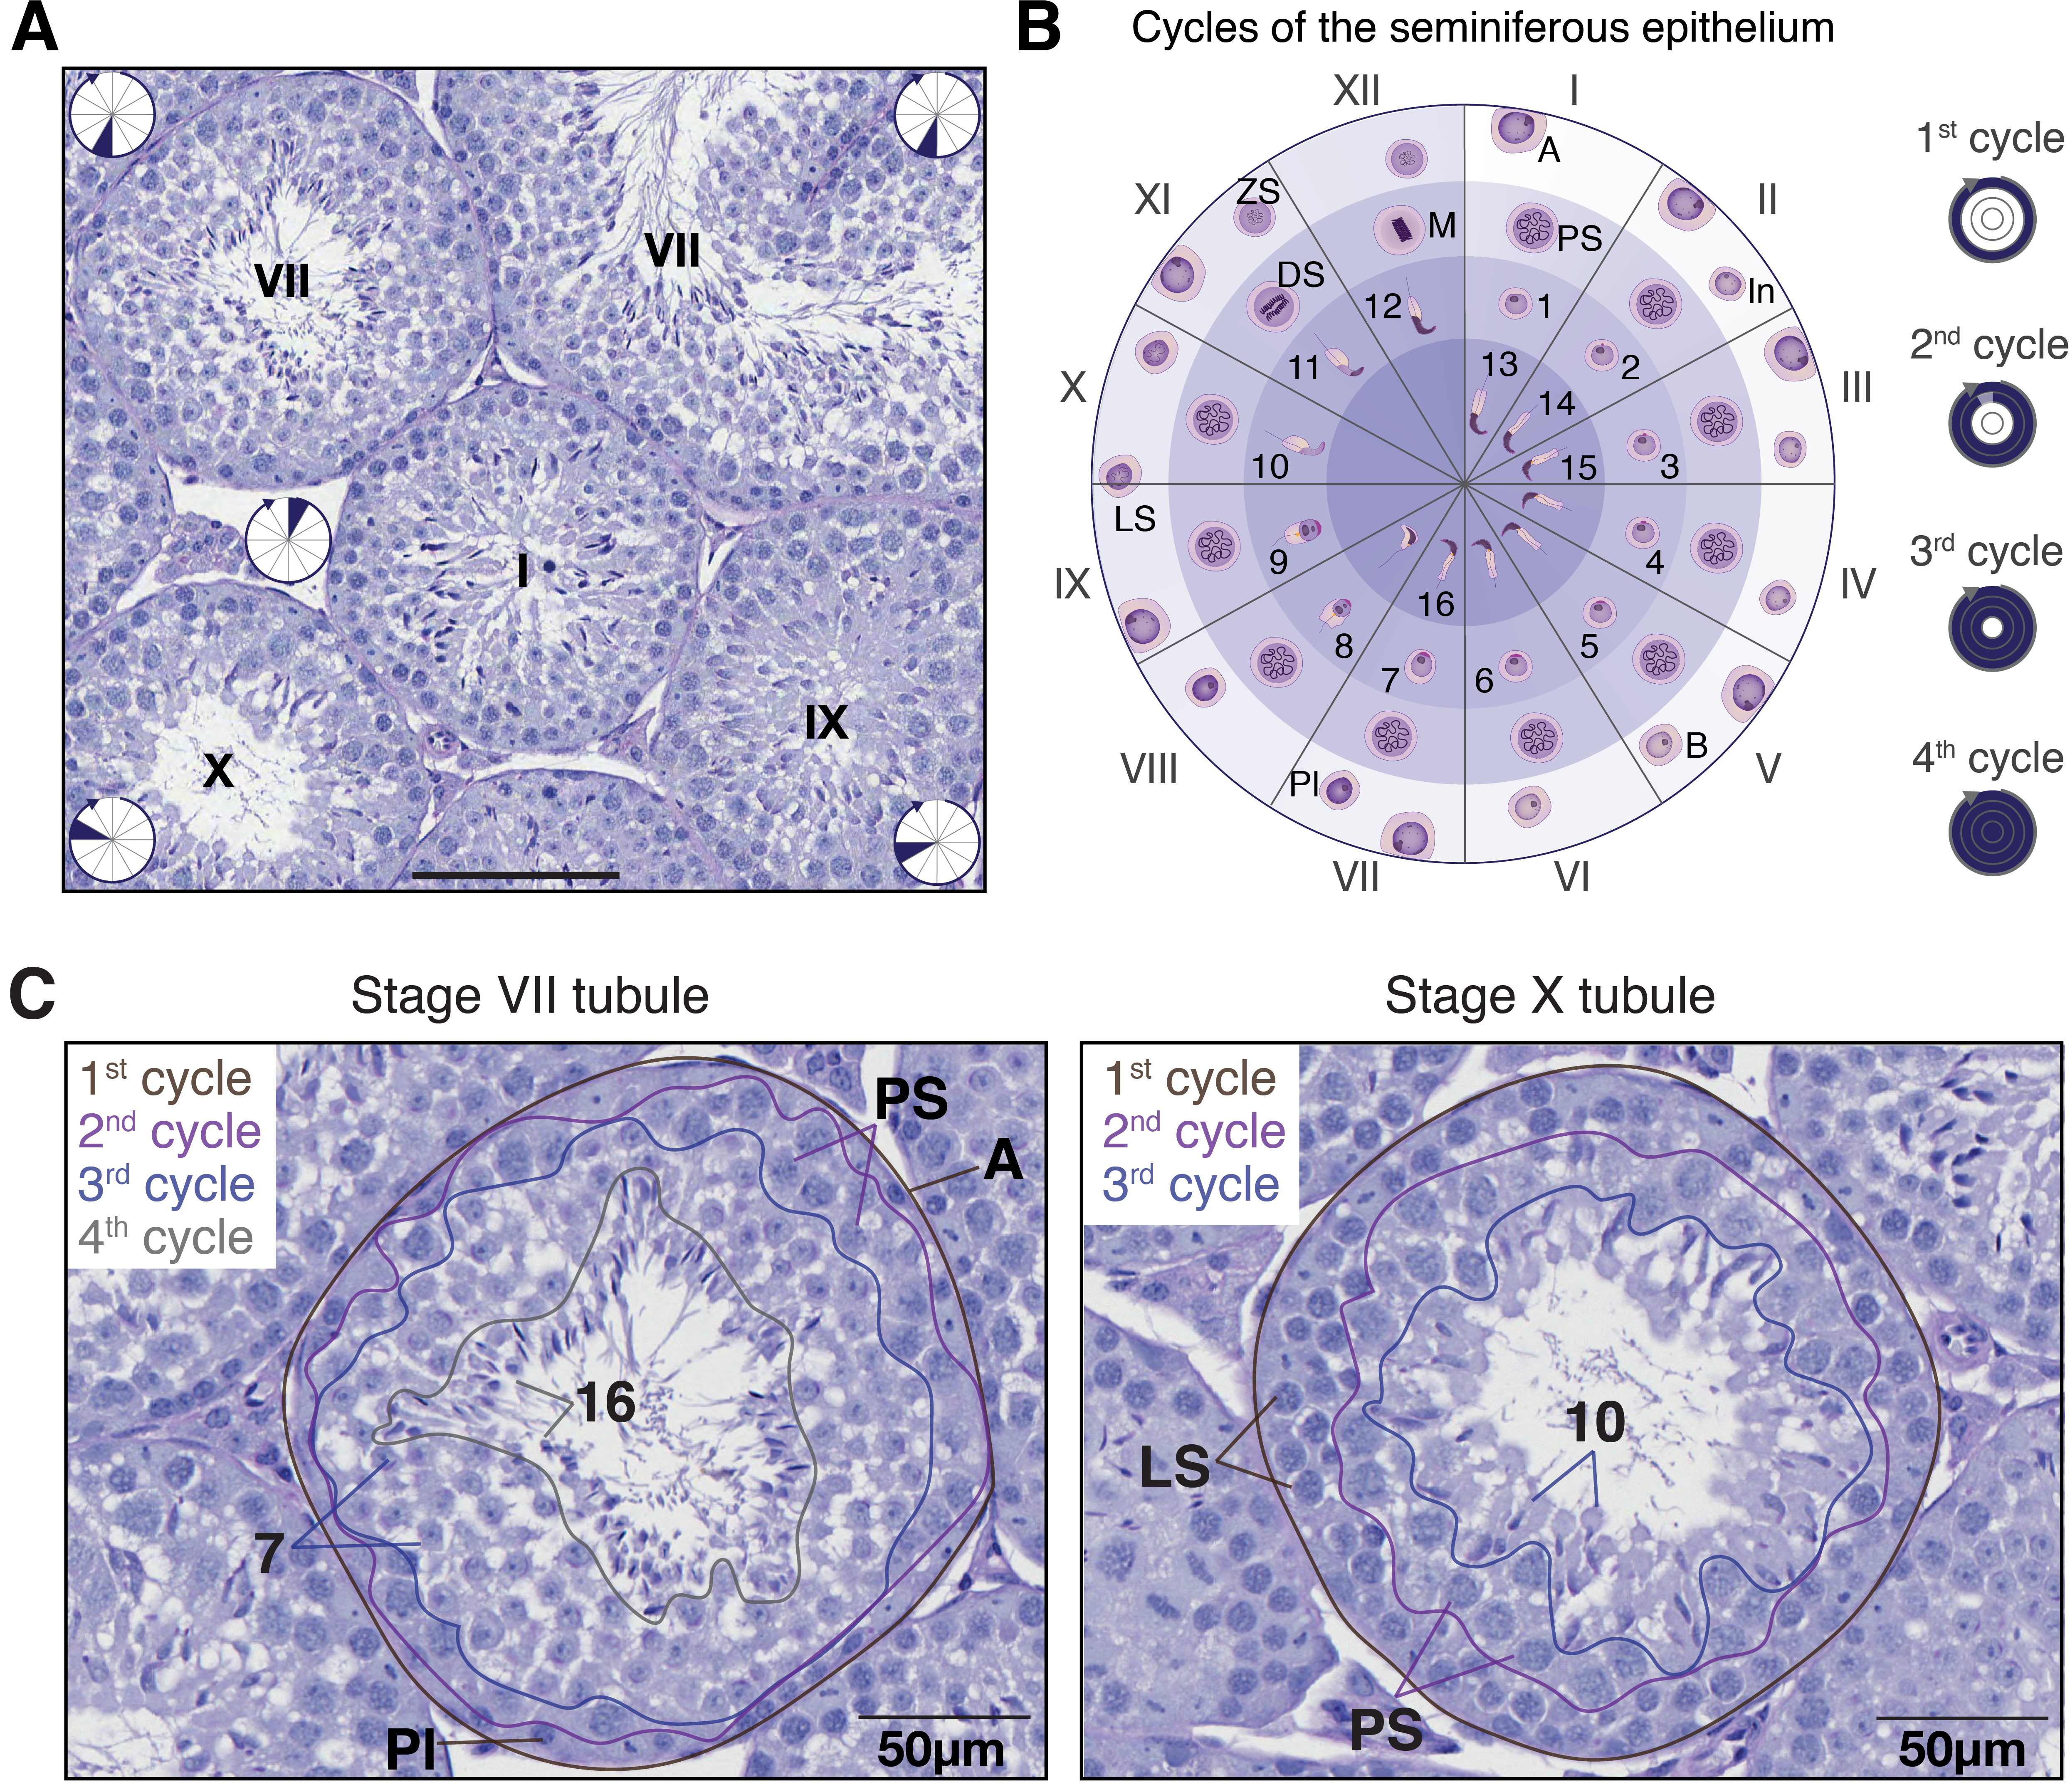
\includegraphics[width=\textwidth]{Fig_1.png}
\caption[Droplet based scRNAseq of mouse spermatogenesis]{\textbf{Single-cell RNA-Seq captures a continuum of germ cell types during adult spermatogenesis. (full legend on next page).}\\}
\label{fig2:cell_types}
\end{figure}

Using multiple functional genomics approaches, we characterized the transcriptional programme underlying mouse spermatogenesis with cells isolated from specifically staged juvenile (between postnatal days 6 and 35) and adult (8-9 weeks) C57BL/6J (B6) mice. For all samples, we generated unbiased droplet-based single-cell RNA sequencing (scRNA-Seq) data from whole testis with matched histology. For this, mouse testes were enzymatically dissociated and single-cell suspensions at a concentration of ~300,000 cells/ml was loaded into one channel of the ChromiumTM Single Cell A Chip (10X Genomics), aiming for a recovery of 4000-5000 cells. Additionally, for juvenile samples, we generated whole-tissue bulk RNA sequencing, as well as mapping chromatin state in purified cell populations using CUT\&{}RUN (Cleavage Under Targets \& Release Using Nuclease) \textbf{(Fig. \ref{fig3:cell_types}C)} \citep{Skene2018}. \\
To obtain gene-specific transcript counts for droplet based scRNA-Seq, the Cell Ranger \emph{count} function with default settings was used to align and count unique molecular identifiers (UMIs) per sample. This software retains cells with similar UMI distributions \citep{Zheng2017}. We use this default threshold to obtain high-quality cells with large numbers of UMIs. After merging all samples, we filtered out cells that express less than 1000 genes. Furthermore, we exclude cells with more than 10\% of reads mapping to the mitochondrial genome. The transcriptomes of quality filtered cells were normalized using the scran package \citep{Lun2016pooling}. After quality control and filtering, we retained a total of 42,796 single cells, 30 bulk RNA-Seq libraries and 8 CUT\&{}RUN libraries \textbf{(Tables \ref{tab3:QC_scRNAseq}-\ref{tab3:QC_CnR})}.

\newpage

\begin{figure}[!h]
\centering
\includegraphics[width=\textwidth]{Fig_2.png}
\caption[Droplet based scRNAseq of mouse spermatogenesis]{\textbf{Single-cell RNA-Seq captures a continuum of germ cell types during adult spermatogenesis. (full legend on next page).}\\}
\label{fig2:cell_types}
\end{figure}

\newpage

\captionsetup[figure]{list=no}
\addtocounter{figure}{-1}   
\captionof{figure}{\textbf{Single-cell RNA-Seq captures a continuum of germ cell types during adult spermatogenesis (continued).}\\
\textbf{(A)} Periodic Acid Schiff (PAS)-stained testis cross-section showing a number of seminiferous tubules at different epithelial stages (displayed as Roman numerals). Within each tubule, the inset circle refers to the corresponding section in (B). Scale bar represents 100 µm; original magnification 200X. \textbf{(B)} Schematic representation of the 12 stages of the seminiferous epithelium in mice. The colour gradient within the circle indicates the differentiation path of germ cells with the layers corresponding to individual cycles of the epithelium. The circle is divided into 12 section, each corresponding to one epithelial stage displaying the characteristic germ cells. Within each section, cells are positioned across the different layers according to their emergence during consecutive cycles, each being 8.6 days apart with more mature cells moving towards the centre.  Cell types are labelled as: A – type A spermatogonia (SG), In – intermediate SG, B – type B SG, Pl – preleptotene spermatocytes (SCs), L – leptotene SCs, Z – zygotene SCs, P – pachytene SCs, D – diplotene SCs, M – metaphase I and II, 1-8 round spermatids, 9-16 elongating spermatids. \textbf{(C)} Overview of the experimental design yielding bulk RNA-Seq, droplet-based scRNA-Seq and chromatin profiling on FACS-purified cells using CUT\&{}RUN from one testis while using the contralateral testis for matched histology. \textbf{(D)} t-distributed stochastic neighbour embedding (tSNE) representation of scRNA-Seq data from adult B6 mice with the colour gradient representing the expression of known marker genes for two somatic cell types and the main germ cell types. The x- and y-axis represent the first and second dimension of tSNE respectively. The colour legend shows log2-transformed, normalized expression counts. \textbf{(E)} Graph-based clustering (see Methods) identifies different sub-stages within major germ cell populations. 
\\}
\captionsetup[figure]{list=yes}


To remove batch-specific effects that arise when samples are prepared and sequenced in different experiments \textbf{(Tables \ref{tab3:QC_scRNAseq})}, we used the \emph{mnnCorrect} function implemented in the \emph{scran} package \citep{Haghverdi2018}. We used the top 1000 genes with highest biological variation across all samples as informative genes for batch correction. The \emph{mnnCorrect} function takes transcriptional profiles of cells isolated from adult B6 mice as first input and uses this dataset as reference for cell mapping.\\

The batch corrected transcriptomes were clustered using a graph-based approach. A shared nearest-neighbour (SNN) graph \citep{Xu2015} was constructed considering 3 shared nearest neighbours using the \emph{buildSNNGraph} function in scran. In the next step, a multi-level modularity optimization algorithm was used to find community structure in the graph \citep{Blondel2008} implemented in \emph{igraph} R package. Clusters were annotated based on the expression of known markers genes. Cells in small clusters that show unclear identities were excluded from down-stream analysis.\\

To find marker genes for each of the identified cell clusters, we performed differential expression testing across multiple pairwise comparisons. To detect cluster-specific marker genes, the \emph{findMarkers} function implemented in \emph{scran} was used on the log$_2$-transformed normalized counts while providing the cluster labels. \\

After clustering all single cell transcriptomes using an unbiased graph-based approach (Methods), we first focused on cells isolated from adult B6 testis to generate a comprehensive map of cell types across spermatogenesis. Using computationally-defined cluster-specific marker genes (Methods; Table S2), we identified the following cell types: spermatogonia (based on Dmrt1 expression, Matson et al., 2010), spermatocytes (Piwil1, Deng and Lin, 2002), round and elongating spermatids (Tex21 and Tnp1, respectively, Fujii et al., 2002), as well as the main somatic cell types of the testis, Sertoli (Cldn11, Mazaud-Guittot et al., 2010) and Leydig cells (Fabp3, Oresti et al., 2013) (Fig. 1D). Using a dimensionality reduction technique for visualization (t-distributed Stochastic Neighbour Embedding; Fig. 1E), the germ cell types from spermatocytes to elongating spermatids formed a continuum, which recapitulated the known developmental trajectory.

\begin{figure}[!h]
\centering
\includegraphics[width=\textwidth]{Fig_3.png}
\caption[Droplet based scRNAseq of mouse spermatogenesis]{\textbf{Single-cell RNA-Seq captures a continuum of germ cell types during adult spermatogenesis. (full legend on next page).}\\}
\label{fig2:cell_types}
\end{figure}



